\section{Theorie}
\label{sec:Theorie}

\subsection{Grundlagen}
Magnetfelder werden durch die Bewegung elektrischer Ladungen erzeugt.
Die magnetische Feldstärke $\vec{H}$ beschreibt die Richtung und Stärke des Magnetfelds.
Der Verlauf des Magnetfeldes kann durch Feldlinien dargestellt werden.
Diese bilden sogenannte Schleifen und sind immer geschlossen.\\
Häufig besitzen Atome allein durch ihre Elektronenanordnung und -bewegung ein dauerhaftes magnetisches Moment.
In dem Fall, dass die magnetischen Momente statistisch verteilt sind, kann die magnetische Flussdichte $\vec{B}$
\begin{equation}
    \vec{B} = \mu \cdot \vec{H}
    \label{eqn:h_zu_b}
\end{equation}
verwendet werden.\\
Dabei ist $\mu$ die Permeabilität und $\vec{H}$ das von außen angelegte Magnetfeld.
$\mu$ ergibt sich aus der Vakuum-Permeabilität $\mu_0$ und der materialabhängigen relativen Permeabilität $\mu_r$
\begin{equation}
    \mu = \mu_0 \cdot \mu_r .
\end{equation}

\subsection{Biot-Savart}
Jeder stromdurchflossener Leiter (z.B. Draht) ist von einem Magnetfeld umgeben. Dieses verläuft in Schleifen, die in einer Ebene
senktrecht zum Stromfluss verlaufen. Das Magnetfeld ergibt sich aus dem Biot-Savartschen Gesetz
\begin{equation}
    \symup{d}\vec{B} = \frac{\mu_0 I}{4\pi} \frac{\symup{d}\vec{s} \times \vec{r}}{r^3}
    \label{eqn:biot}
\end{equation}
mit der Magnetfeldstärke $\vec{B}$ bei dem Abstand $r$ vom Draht, welcher mit einem Strom $I$ durchflossen wird.

\subsection{Leiterschleifen}
Das Biot-Savart-Gesetz wird nun verwendet um das Magnetfeld einer Leiterschleife zu berechnen. Eine Leiterschleife
kann als Spule mit $n=1$ Windungen angesehen werden. Im Mittelpunkt des stromdurchflossenen Ringes folgt aus dem Biot-Savart-Gesetz\eqref{eqn:biot}
\begin{equation}
    \vec{B}(x) = \frac{\mu_0 I}{2} \frac{R^2}{(R^2+x^2)^(3/2)} \cdot \hat{x}
\end{equation}
für die Magnetfeldstärke. Hier beschreibt $x$ den Abstand zur Ringmitte und $R$ den Radius des Kreisrings.  \\

\subsection{Spulen}
Bei einem Solenoid (zylindrische Spule) verlaufen die Feldlinien innerhalb der Spule parallel zum Spulenrand. Das Magnetfeld ist in der Spulenmitte homogen und konstant.
Außerhalb der Spule verlaufen die Feldlinien in geschlossenen Schleifen. Das Feld ist hier inhomogen.\\
Die magnetische Feldstärke einer langen Spule berechnet sich durch
\begin{equation}
    B = \mu_r \mu_0 \frac{n}{l} I
\end{equation}
mit der Windungszahl $n$ und der Spulenlänge $l$.\\

\subsection{Helmholtz-Spule}
Wird ein homogenes Magnetfeld benötigt, so werden häufig zwei gleiche Spulen mit Radius $R$ verwendet.
Die Spulen stehen gegenüber mit dem Abstand $d=R$ (siehe \ref{fig:helmholtz}). Das Magnetfeld in der Mitte der Symmetrieachse eines Helmholtz-Spulenpaar mit $n=1$ Windungen wird durch
\begin{equation}
    B(0) = B_1(x) + B_1(-x) = \frac{\mu_0 I R^2}{(R^2+x^2)^{3/2}}
\end{equation}
beschrieben.
\begin{figure}
    \centering
    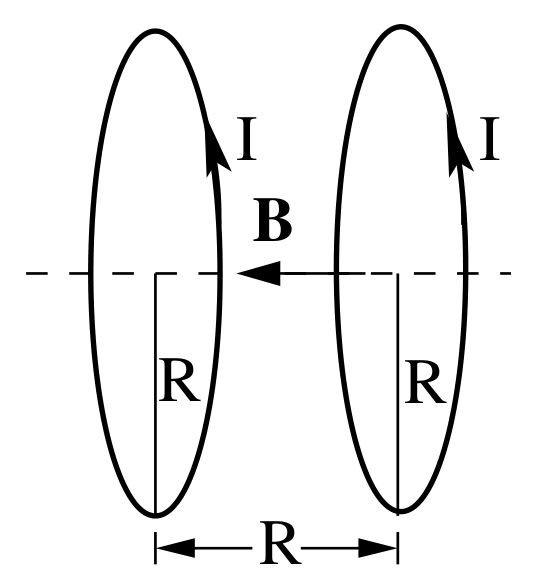
\includegraphics[height=4.5cm]{content/helmholtz.jpg}
    \caption{Helmholtz-Spulenpaar mit Radius $R$ und Abstand $d=R$. \cite[2]{anleitung}}
    \label{fig:helmholtz}
\end{figure}
\\
Der allgemeine Fall für eine Spule mit $n$ Windungen und beliebigen Abstand $d$ wird durch die Formel 
\cite[87--88]{demtroeder}
\begin{equation}
    B(z) = \frac{\mu_0 \cdot I \cdot R^2}{2} \cdot \left ( \frac{1}{\left((z+d/2)^2+R^2\right)^{3/2}} + \frac{1}{\left((z-d/2)^2+R^2\right)^{3/2}} \right )
    \label{eqn:helm}
\end{equation}
beschrieben.

\subsection{Ferromagnetismus}
Die Magnetisierung eines Körpers setzt sich aus vielen kleinen Magnetisierungen, wie Ionen und quasifreie Elektronen zusammen.
Ferromagnetismus beschreibt Material, welches auch ohne äußeres Feld ein magnetisches Moment besitzt (z.B. Eisen).\\
Wird ein äußeres Magnetfeld angelegt, so richten sich die magnetischen Momente in sogenannten Weiß'schen Berirken zueinander aus,
bis alle Weiß'schen Bezirke parallel zum Magnetfeld stehen. Wird das äußere Magnetfeld abgeschaltet so besitzt das Material weiterhin
ein magnetisches Moment. Die relative Permeabilität $\mu_r$ ist sehr groß und die Gleichung \eqref{eqn:h_zu_b} beschreibt nicht mehr
das Magnetfeld $B$.\\

\subsection{Hysterese-Kurve}
Die Änderung der Magnetisierung kann durch die Hysterese Kurve dargestellt werden. Der Verlauf der Kurve ist materialabhängig und
variiert mit der Vorgeschichte des Materials.\\ \\
Bei einem zuvor unmagnetisiertem Material sind die Weiß'schen Bezirke ohne äußeres Magnetfeld zufällig verteilt. Wird nun ein äußeres Feld angelegt so
steigt die Magnetisierung bis zum Sättigungswert $B_s$ (siehe Abbildung \ref{fig:hysterese}: Neukurve (1)). Hier sind alle Weiß'schen Bezirke parallel ausgerichtet.\\
Wird jetzt das äußere Magnetfeld abgeschaltet, so bleibt eine Restmagnetisierung, die Remanenz $B_r$ (siehe Abbildung \ref{fig:hysterese}: (2)).
Mithilfe der Koerzitivkraft $H_c$ (ein magnetisches Gegenfeld) kann die Remanenz aufgehoben werden und die Magnetisierung beträgt wieder null.\\
Wird nun weiter das äußere Magnetfeld erhöht, so nähert sich die Magnetisierung dem Sättigungswert $-B_s$. Zum Schluss wird das Magnetfeld wieder abgeschaltet und ein Magnetfeld,
wie am Anfang angelegt (siehe Abbildung \ref{fig:hysterese}: (3)).
\begin{figure}
    \centering
    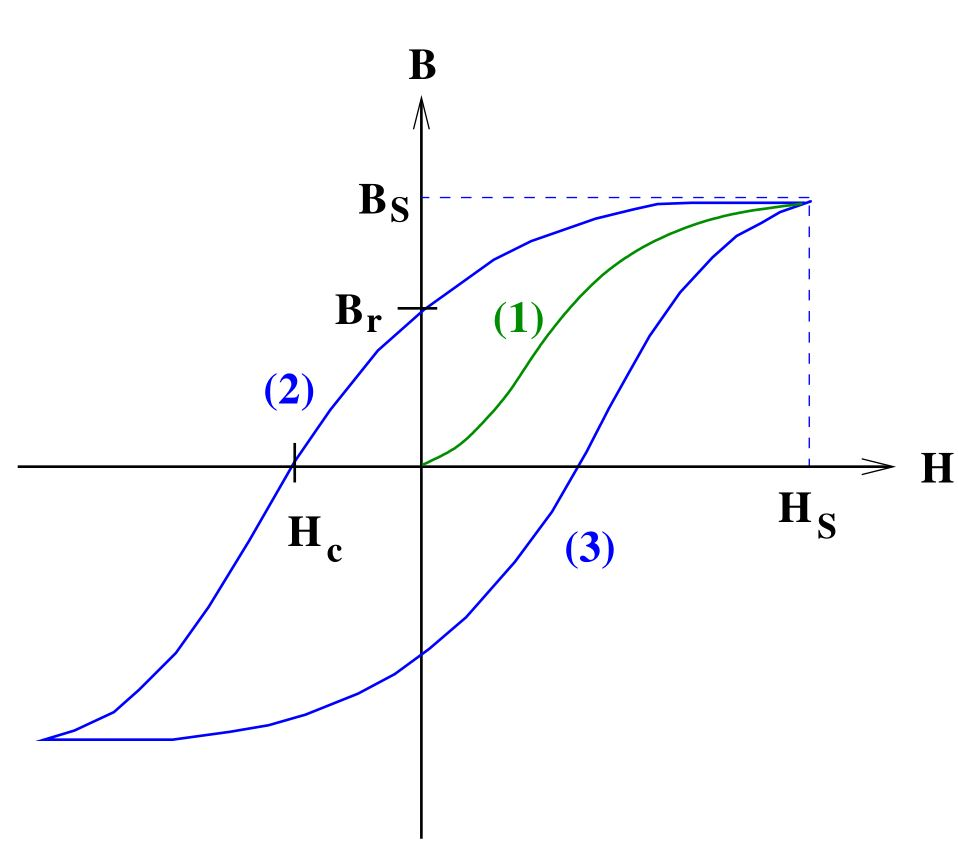
\includegraphics[height=6cm]{content/hysterese.jpg}
    \caption{Die Hysterese-Kurve zeigt den Verlauf der Magnetisierung eines ferromagnetischen Stoffes. \cite[3]{anleitung}}
    \label{fig:hysterese}
\end{figure}
\\
\\
Wie in der Abbildung \ref{fig:hysterese} zu sehen, muss $\mu_r$ eine Funktion der Feldstärke $H$ sein.
Die differentielle Permeabilität
\begin{equation}
    \mu_\text{diff} = \frac{1}{\mu_0} \frac{\symup{d}B}{\symup{d}H}
\end{equation}
beschreibt die Neukurve(1). Allgemein wird der magnetische Fluss einer Spule mit Eisenkern durch
\begin{equation}
    \vec{B} = \mu_0 \left( \vec{H} + \vec{B} \right)
\end{equation}
beschrieben, wobei $\vec{M}$ für die Magnetisierung des Materials steht.